
\section{Xアームの基線長伸縮}



\subsection{同相成分と逆相成分}
図\ref{img:img_diffcomm}で示すような,Xアーム上の2点,$x_1,\,x_2$を考える。それぞれの場所での変位は変位場$u(x,t)$をもちいて,$u(x_1,t),u(x_2,t)$となる。ここで,これら2つの変位の同相成分$u_{\mathrm{com}}$と逆相成分$u_\mathrm{diff}$を
\begin{eqnarray}\label{eq:eq22}
  u_{\mathrm{diff}} &\equiv& \frac{u_{1}-u_{2}}{\sqrt{2}}, \\
  u_{\mathrm{com}}  &\equiv& \frac{u_{1}+u_{2}}{\sqrt{2}}
\end{eqnarray}
と定義する。パワーが保存するように、規格化定数は$\sqrt{2}$にしている。同相成分は,2点の重心移動をあらわし,逆相成分は2点の基線長伸縮を表す。


\begin{figure}[H]
  \begin{center}
    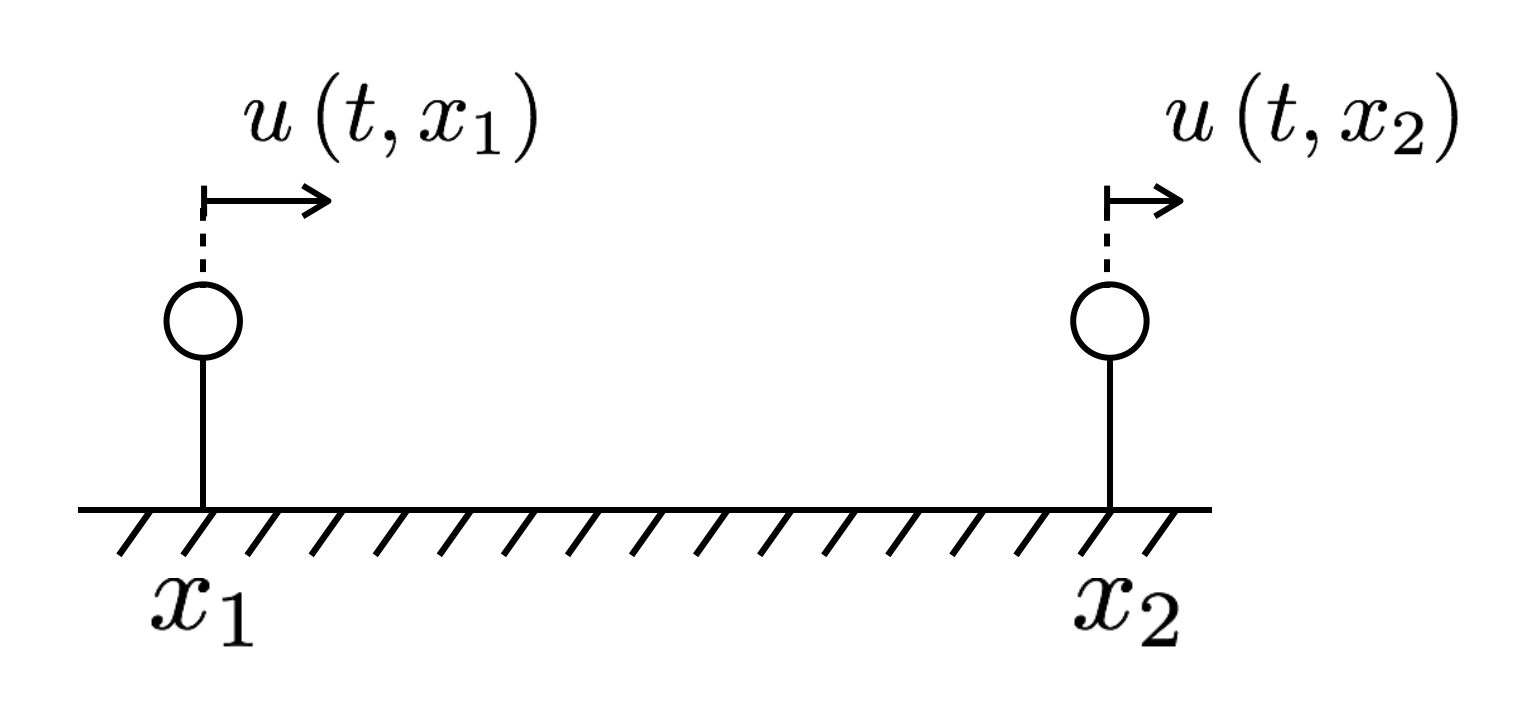
\includegraphics[width=11.5cm]{./img_cdmr_xarm.png}
  \end{center}
  \caption{Xアーム上の2点の変位。それぞれの位置を$x_1,\,x_2$とすれば変位はそれぞれ$u(x_1,t),\,u(x_2,t)$となる。}\label{img:img_diffcomm}
\end{figure}


\subsection{Common Differential Mode Rate (CDMR)}
2点の逆相成分である,基線長伸縮がどの程度低減されているかを表す指標として,2つの信号の同相と逆相の振幅成分の比、Common Differential Mode Rate (CDMR) を
\begin{equation}
  \boxed{\mathrm{CDMR} \equiv \sqrt{\frac{同相成分のパワー}{逆相成分のパワー}} = \sqrt{\frac{P_{\mathrm{com}}(\omega)}{P_{\mathrm{diff}}(\omega)}}} \label{eq:eq23}
\end{equation}
と定義する。\footnote[0]{きっかけは道村さんからの4月19日のメール「KAGRA micro seismのコヒーレンス」に対する回答になる。質問の内容は,「脈動では,数kmのXアームはどれだけ同相成分を含んでいて,どれだけ逆相成分を低減できているか」というもの。経験的に,IMCのような数10mスケールの基線長では,よく逆相成分が低減されているいることが知られている。なので,基線長が長くなると同相成分と逆相成分の比がどう変わるのか。それを評価した。}
$P_{\mathrm{com}},P_{\mathrm{diff}}$は同相成分と逆相成分についてのパワースペクトル密度である。パワースペクトル密度は自己相関関数$C(\tau)$をフーリエ変換したものなので、まず自己相関関数$C_{\mathrm{diff}}$を求める。自己相関関数$C_{\mathrm{diff}}$は,各々の自己相関を$ C_{ij} \equiv \langle x_{i}(t)x_{j}(t+\tau)\rangle,\, (i=1,2,\,j=1,2)$と定義すれば, 
\begin{eqnarray}
  C_{\mathrm{diff}}(\tau) &=& \frac{1}{2}
  \langle
  \left[ x_{1}(t)-x_{2}(t) \right]   \left[ x_{1}(t+\tau)-x_{2}(t+\tau) \right]
  \rangle \\
  &=& \frac{1}{2}\left( C_{11}(\tau) - C_{12}(\tau) - C_{21}(\tau) + C_{22}(\tau) \right), 
\end{eqnarray}
となるので、これをフーリエ変換すれば逆相成分のパワースペクトル密度$P_{\mathrm{diff}}(\omega)$は
\begin{eqnarray}
  P_{\mathrm{diff}}(\omega) &=& \frac{1}{2}\left( P_{1}(\omega) + P_{2}(\omega) - X_{12}(\omega) - X_{12}^*(\omega) \right)\\
  &=& \frac{1}{2} \sqrt{P_{1}P_{2}} \left( \sqrt{\frac{P_{1}}{P_{2}}}+ \sqrt{\frac{P_{2}}{P_{1}}} - 2\Re \left[\mathrm{coh} \right] \right) , 
\mathrm{coh} \equiv \frac{X_{12}}{\sqrt{P_{1}P_{2}}} \label{eq:eq31}
\end{eqnarray}
となる。$P_{1}(\omega),P_{2}(\omega)$はパワースペクトル密度、$X_{12}(\omega)$はクロススペクトル密度、$\mathrm{coh}$はコヒーレンスである。


さて、2つの信号$x_{1},x_{2}$のパワーが同じ、つまり$P_{1}=P_{2}\equiv P$の場合、式(\ref{eq:eq31})はさらに計算できて、結果として$P_{\mathrm{diff}}$は
\begin{eqnarray}
 P_{\mathrm{diff}}(\omega) = P \left(1 - \Re \left[\mathrm{coh} \right] \right) \label{eq:eq35}
\end{eqnarray}
となる。同相成分も同様の計算をして、
\begin{eqnarray}
 P_{\mathrm{com}}(\omega) = P \left(1 + \Re \left[\mathrm{coh} \right] \right) \label{eq:eq36}
\end{eqnarray}
となるので、$\mathrm{CDMR}$は定義式(\ref{eq:eq23})より、
\begin{eqnarray}
 \mathrm{CDMR} = \sqrt{\frac{1 + \Re \left[\mathrm{coh} \right] }{1 - \Re \left[\mathrm{coh} \right]}} \label{eq:eq33}
\end{eqnarray}
と書き表すことができる。
式(\ref{eq:eq33})が示すように、同相成分と逆相成分のパワー比は2つの信号のコヒーレンスであらわすことができる。


\subsubsection{平面波モデル($\mathrm{CDMR_{seis}}$)}
図\ref{img:img_diffcomm}を平面波が伝搬している場合のCDMRを求める。変位場$u(x,t)$は、角周波数$\omega$と波数$k$を用いて、
\begin{equation}
  u(x,t) = u_{0}e^{i(\omega{t}-k{x})}
\end{equation}
と表すことができる。$u_{0}$は$t=0,x=0$での変位である。図\ref{img:img_diffcomm}において、$x_2$にある点がもう一つの点$x_1$にたいして,$x_2=x_1+L$離れているとすると、
これらの逆相成分$u_{\mathrm{diff}}(x,t)$は
\begin{eqnarray}
  u_{\mathrm{diff}}(x,t) &=& \frac{1}{\sqrt{2}}\left( e^{i(\omega{t}-k{x_1})} -e^{i(\omega{t}-k{x_1+kL})} \right)\\
  &=& \frac{1}{\sqrt{2}}u(x_1,t)\left( 1-e^{ikL)}  \right)\\
  &=& u(x_1,t)\times{\sqrt{2}{(-i)}}e^{i\frac{kL}{2}}\mathrm{sin}(\frac{kL}{2})
\end{eqnarray}
となる。同相成分$u_\mathrm{com}(x,t)$も同様の計算をして,
\begin{equation}
  u_{\mathrm{com}}(x,t) = u(x_1,t)\times{\sqrt{2}}e^{i\frac{kL}{2}}\mathrm{cos}(\frac{kL}{2})
\end{equation}
となるので,平面波が通過しているときの$\mathrm{CDMR}$は
\begin{equation}
  \boxed{\mathrm{CDMR_{seis}} = \left| \frac{u(x_1,t)\times{\sqrt{2}}e^{i\frac{kL}{2}}\mathrm{cos}(\frac{kL}{2})}{u(x_1,t)\times{\sqrt{2}{-i}}e^{i\frac{kL}{2}}\mathrm{sin}(\frac{kL}{2})}  \right| = \frac{1}{\mathrm{tan\left( \frac{\omega{L}}{2c}  \right)}}}
  \label{eq:eq18}
\end{equation}
で表すことができる。ここで,平面波の分散関係$c=\omega/k$を用いた。


\subsubsection{平面波モデル($\mathrm{CDMR_{gif}}$)}
GIFと地震計を比較するために、式\ref{eq:eq23}の逆相成分をGIFのひずみ計で置き換えた$\mathrm{CDMR_{gif}}$を計算する。GIFのひずみ計は1500m離れた2点間のひずみ$\varepsilon_{\mathrm{gif}}$を測っている。そのため,3km離れた二点の地面振動の逆相成分$x_{\mathrm{diff_{gif}}}$は,
\begin{equation}
  x_{\mathrm{diff_{gif}}} = \varepsilon_{\mathrm{gif}}\times \frac{3000}{\sqrt{2}}\label{eq:eq34} 
\end{equation}
と換算することができる。\footnote[5]{数kmスケールの基線長のひずみ応答は数Hzまで平坦なので,脈動以下の周波数帯域では,単純にスケール倍すればいい。}


平面波が伝搬しているとき,速度$v(x,t)$は$v(x,t) \equiv \frac{\partial{u}}{\partial{t}} = i\omega{u(x,t)}$であり、ひずみ$\epsilon(x,t) $ は$\epsilon(x,t) \equiv \frac{\partial{u}}{\partial{x}} = -ik{u(x,t)}$となるので、両者の振幅比は

\begin{equation}
  \left| \frac{A_v}{A_\epsilon} \right|= c \label{eq:eq40}
\end{equation}
となって,位相速度$c$で表すことができる。


さて,GIFで逆相成分を置き換えた$\mathrm{CDMR_{gif}}$は、式\ref{eq:eq36}と式\ref{eq:eq34}をもちいて、
\begin{eqnarray}
\mathrm{CDMR_{\mathrm{gif}}} = \frac{ u(x_1,t)\times{\sqrt{2}}e^{i\frac{kL}{2}}\mathrm{cos}(\frac{kL}{2})  }{{A_{\epsilon}L}/{\sqrt{2}}}  \label{eq:eq37} 
\end{eqnarray}
となるが、コヒーレンスは$\mathrm{coh}=e^{ikL}$なので、計算すると
\begin{empheq}[box=\fbox]{align}
  \mathrm{CDMR_{\mathrm{gif}}} = \sqrt{2\left(1+cos(kL)\right)}\frac{A_{v}}{A_{\epsilon}}\frac{\omega}{L} = \frac{{2c}}{\omega{L}}\mathrm{cos}(\frac{\omega{L}}{{2c}}) \label{eq:eq39} 
\end{empheq}
となる。


\subsection{地震計のノイズ}\label{nm}
\subsubsection{コヒーレンスをつかったノイズ評価}
\begin{figure}[H]
  \begin{center}
    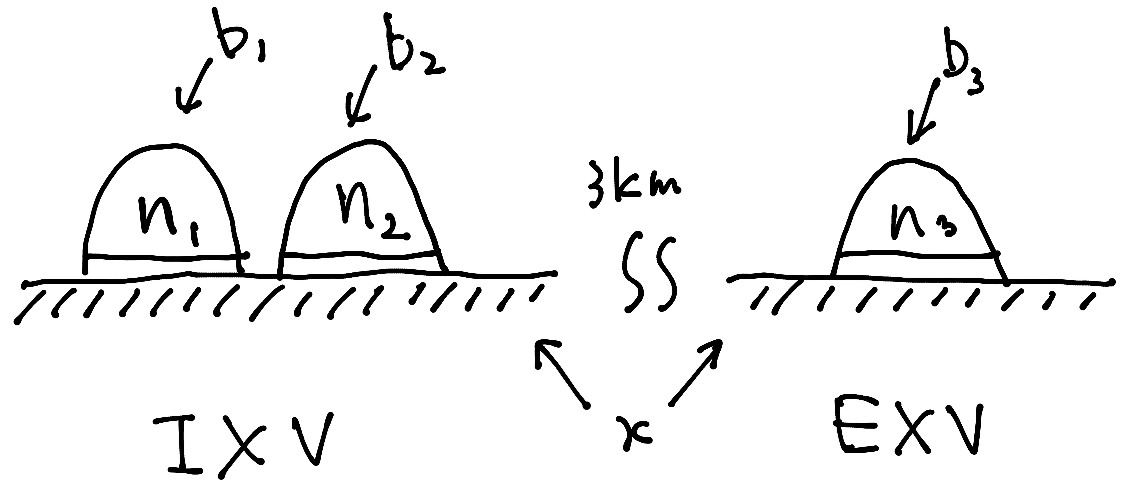
\includegraphics[width=8.5cm]{./img_noisemeasurement.png}
  \end{center}
  \caption{ノイズ測定のための地震計の配置。IXVには2台の地震計を隣接して設置し、EXVには1台の地震計を設置する。$n_1,n_2,n_3$は地震計のSelfNoise、$b_1,b_2,b_3$はローカルな環境ノイズ。$x$は地面振動。IXVにある地震計2つは隣接しているので$b_1=b_2=b$とする。また今回の足的では同じTrillium120QAを使っているので、$n_1=n_2=n_3=n$とした。
  }\label{img:img_noisemeasurement}
\end{figure}

地震計のノイズは低周波になればなるほど増大するため、とくに静かなサイトでは、ノイズが地面振動を上回ってしまい計測を制限する。


信号とノイズを区別する方法としてコヒーレンスを用いたものがある\cite{peterson1980test}。この方法はランダムノイズとコモンモードノイズを区別する場合に有効であり、地震計に限らず他のセンサーに適用することができる\cite{barzilai1998technique}。たとえば2台の同一の地震計を隣接して置けば、地面振動はコモンモードノイズとして現れ、地震計内部から生じるSelfNoiseはインコヒーレントなノイズなので、両者を区別することができる。しかし隣接して設置するとローカルな環境ノイズもコモンモードノイズとして現れるため、地面振動と区別することができない。そこでローカルな環境ノイズがインコヒーレントになるよう、半れた場所に地震計を置くと、環境ノイズと地面振動は区別できる。このようにすれば、地面振動と環境ノイズ、SelfNoiseを区別し評価することができる。


Trillium120QAのノイズ評価のための実験セットアップを図\ref{img:img_noisemeasurement}に示す。Yエンドの地震計をセンターに運び、センターに2台、Xエンドに1台用意する。このとき、低周波地面振動はセンターとXエンドでコヒーレントな信号であり、$x$とする。さらにSelfNoiseを$n_i$、ローカルな環境の外乱を$b_i$とする。添字の$i$は(IXV,EYV,EXV)に対応する。センターの2台は隣接しているので環境ノイズはコモンモードノイズとなり$b_1=b_2\equiv b$とする。さらに同一の測定装置で計測するので$n_1=n_2\equiv n$とする。一方でXエンドはADCノイズで高周波が制限されないよう30dbのプリアンプを通しているので、SelfNoiseの入力換算ノイズはIXVとEYVと異なり、$n_3\neq n_1,n_3\neq n_2$である。


上述したように、地面振動と環境ノイズ、SelfNoiseを互いに区別するためには少なくとも2つの測定を行わなければならない。それらを測定A、測定Bとして後述する。


\subsubsection{測定A:SelfNoiseの評価}
\begin{figure}[H]
  \begin{center}
    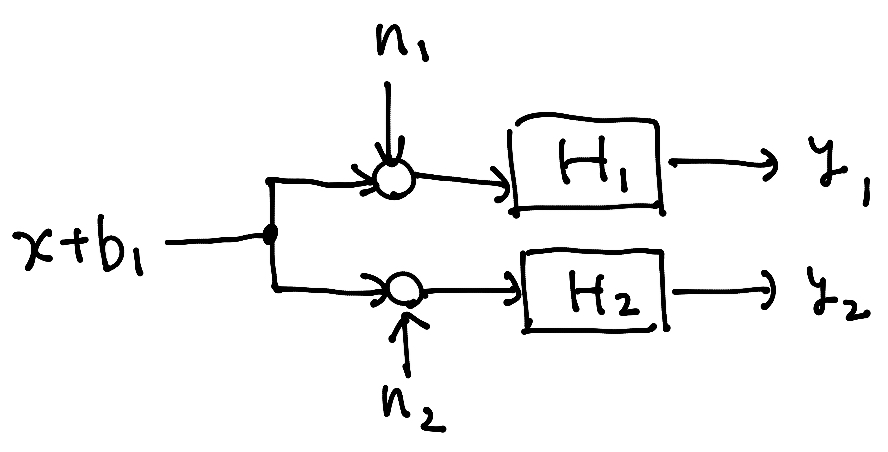
\includegraphics[width=8.5cm]{./img_noisemeasurement_testa.png}
  \end{center}
  \caption{
  }\label{img:img_testA}
\end{figure}

測定Aでは隣接した地震計2つのコヒーレンスを求める。ブロック図を図\ref{img:img_testA}に示す。このときの地震計の出力信号はそれぞれ、
\begin{eqnarray}
  Y_{1}(\omega) &=& \left| H_{1}(i\omega)\right|^{2}\left[X(\omega)+B(\omega)+N(\omega) \right] \label{eq:eq_nm1} \\ 
  Y_{2}(\omega) &=& \left| H_{2}(i\omega)\right|^{2}\left[X(\omega)+B(\omega)+N(\omega) \right] \label{eq:eq_nm2}
\end{eqnarray}
となる。$Y(\omega),\,X(\omega),\,B(\omega),\,N(\omega)$はそれぞれ$y(t),\,x(t),\,b(t),\,n(t)$のパワースペクトル密度関数であり、$H_1(i\omega),\,H_2(i\omega)$はそれぞれ地震計1,2の伝達関数である。
SelfNoiseは無相関なので、地震計1,2のクロススペクトル密度関数$Y_{12}$は、
\begin{eqnarray}
Y_{12}(i\omega) &=& H_{1}(i\omega)H_{2}^{*}(i\omega)\left[X(\omega)+B(\omega) \right] 
\end{eqnarray}
のように表すことができ、2乗コヒーレンス$\gamma_{12}^{2}$は,
\begin{eqnarray}
  \gamma_{12}^{2} &=& \frac{\left| Y_{12}(i\omega)\right|^{2}}{Y_1(\omega)Y_1({\omega})}\\
  &=& \frac{\left | H_{1}(i\omega)H_{2}^{*}(i\omega)\left[X(\omega)+B(\omega) \right] \right |^{2}}{\left| H_{1}(i\omega)^{2}\right|\left|H_{2}(i\omega)\right|^{2}\left[X(\omega)+B(\omega)+N(\omega) \right]^{2}}\\
  &=& \left( \frac{X(\omega)+B(\omega)}{X(\omega)+B(\omega)+N(\omega)} \right)^{2}\\
    &=& \left( \frac{\mathrm{SNR}}{1+\mathrm{SNR}} \right)^{2}\label{eq:eq_nm3}
\end{eqnarray}
となる。
ここで$\mathrm{SNR}$は信号雑音比であり、$\mathrm{SNR}\equiv \frac{X(\omega)+B(\omega)}{N{\omega}}$と定義した。このSNRはコヒーレンスがある信号とコヒーレンスがない信号の比になっている。式(\ref{eq:eq_nm3})より$\mathrm{SNR}$は2乗コヒーレンス$\gamma^{2}_{12}$で求めることができる。

式(\ref{eq:eq_nm1})を用いると、コヒーレンスがないSelfNoise成分とコヒーレンスがある信号成分が以下のように求まる。
\begin{eqnarray}
  N(\omega) &=& \frac{Y_{1}(\omega)}{\left| H_{1}(i\omega) \right|}\frac{1}{1+\mathrm{SNR}} \label{eq:eq_nm4}\\
  X(\omega) + B(\omega) &=& \frac{Y_{1}(\omega)}{\left| H_{1}(i\omega) \right|}\frac{1}{(1+\mathrm{SNR})\mathrm{SNR}} \label{eq:eq_num5}
\end{eqnarray}
測定Aではローカルな環境ノイズ$B(\omega)$がコヒーレンスを持っているためグローバルな地面振動$X({\omega})$と区別ができない。そのため環境ノイズがコヒーレンスを持たないよう十分離れた位置にある地震計とコヒーレンスを取り、地面振動と環境ノイズを分離する必要がある。これを測定Bとする。


\subsubsection{測定B:ローカルな環境ノイズの評価}
\begin{figure}[H]
  \begin{center}
    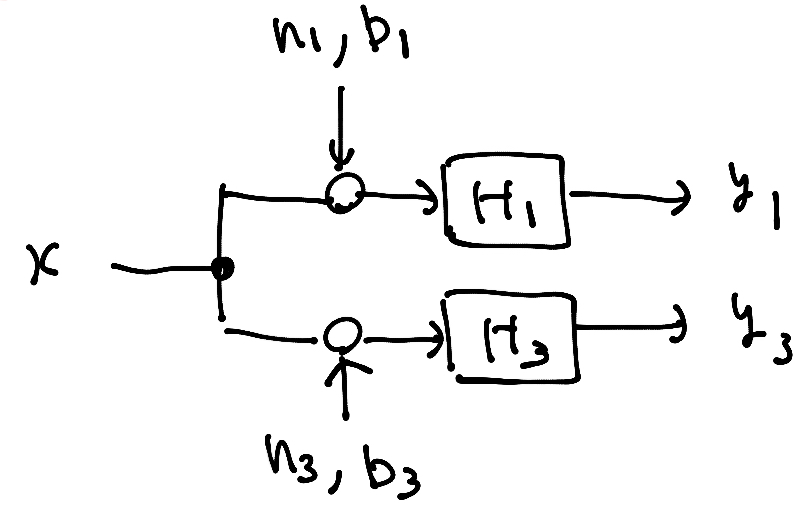
\includegraphics[width=8.5cm]{./img_noisemeasurement_testb.png}
  \end{center}
  \caption{
  }\label{img:img_testB}
\end{figure}

測定BではIXVにおいた地震計1とEXVにおいた地震計3のコヒーレンスを求める。図\ref{img:img_testB}にブロック図を示す。測定Aとは異なり、ローカルな環境ノイズは相関を持たないため地震計1と地震計3のクロススペクトル密度関数$Y_{12}(i\omega)$は
\begin{eqnarray}
Y_{13}(i\omega) &=& H_{1}(i\omega)H_{3}^{*}(i\omega)\left[X(\omega) \right] \\ 
\end{eqnarray}
となる。したがって2乗コヒーレンス$\gamma_{13}^{2}$は,
\begin{eqnarray}
  \gamma_{13}^{2} &=& \frac{\left| Y_{13}(i\omega)\right|^{2}}{Y_1(\omega)Y_3({\omega})}\\
  &=& \frac{\left | H_{1}(i\omega)H_{3}^{*}(i\omega)\right|^{2}X(\omega)^{2}}{Y_1(\omega)Y_3({\omega})}\label{eq:eq_num6}
\end{eqnarray}
となる。したがって、$X(\omega)$は
\begin{eqnarray}
  X(\omega) &=& \frac{\gamma_{13}}{\left | H_{1}(i\omega)H_{3}^{*}(i\omega)\right|}
  \sqrt{Y_1(\omega)Y_3({\omega})} \label{eq:eq_num7}
\end{eqnarray}
となる。式(\ref{eq:eq_num7})と式(\ref{eq:eq_num5})より、$B(\omega)$が求まる。


以上のようにして、地面振動$X(\omega)$とSelfNoise$N(\omega)$を区別することができる。


\subsection{XアームのCDMR}
XアームのCDMRを求める。エンドとセンターの2階においた地震計のXアーム方向の信号をつかった。

\subsubsection{地震計のスペクトル}
まず図\ref{img:img1}に、Xエンドとセンターに置いた地震計の出力を変位にしたAmplitude Spectrum Density (ASD)を示す。0.1-0.3Hzの帯域では大きさが一致している。それ以上の周波数では、センターエリアに置いた地震計はADCノイズで埋もれているため、両者は一致しない。\footnote[6]{プリアンプを入れる予定。KAGRAでよういされているホワイトニングフィルターが横澤さんのおかげで使えるのでそれをつかう。Xエンドはそれをつかっている。。}また低周波では、傾き成分のカップリングにより両者は一致していない。\footnote[7]{積極的に,傾きのカップリングだとは言えない気がする。}

\begin{figure}[H]
  \begin{center}
    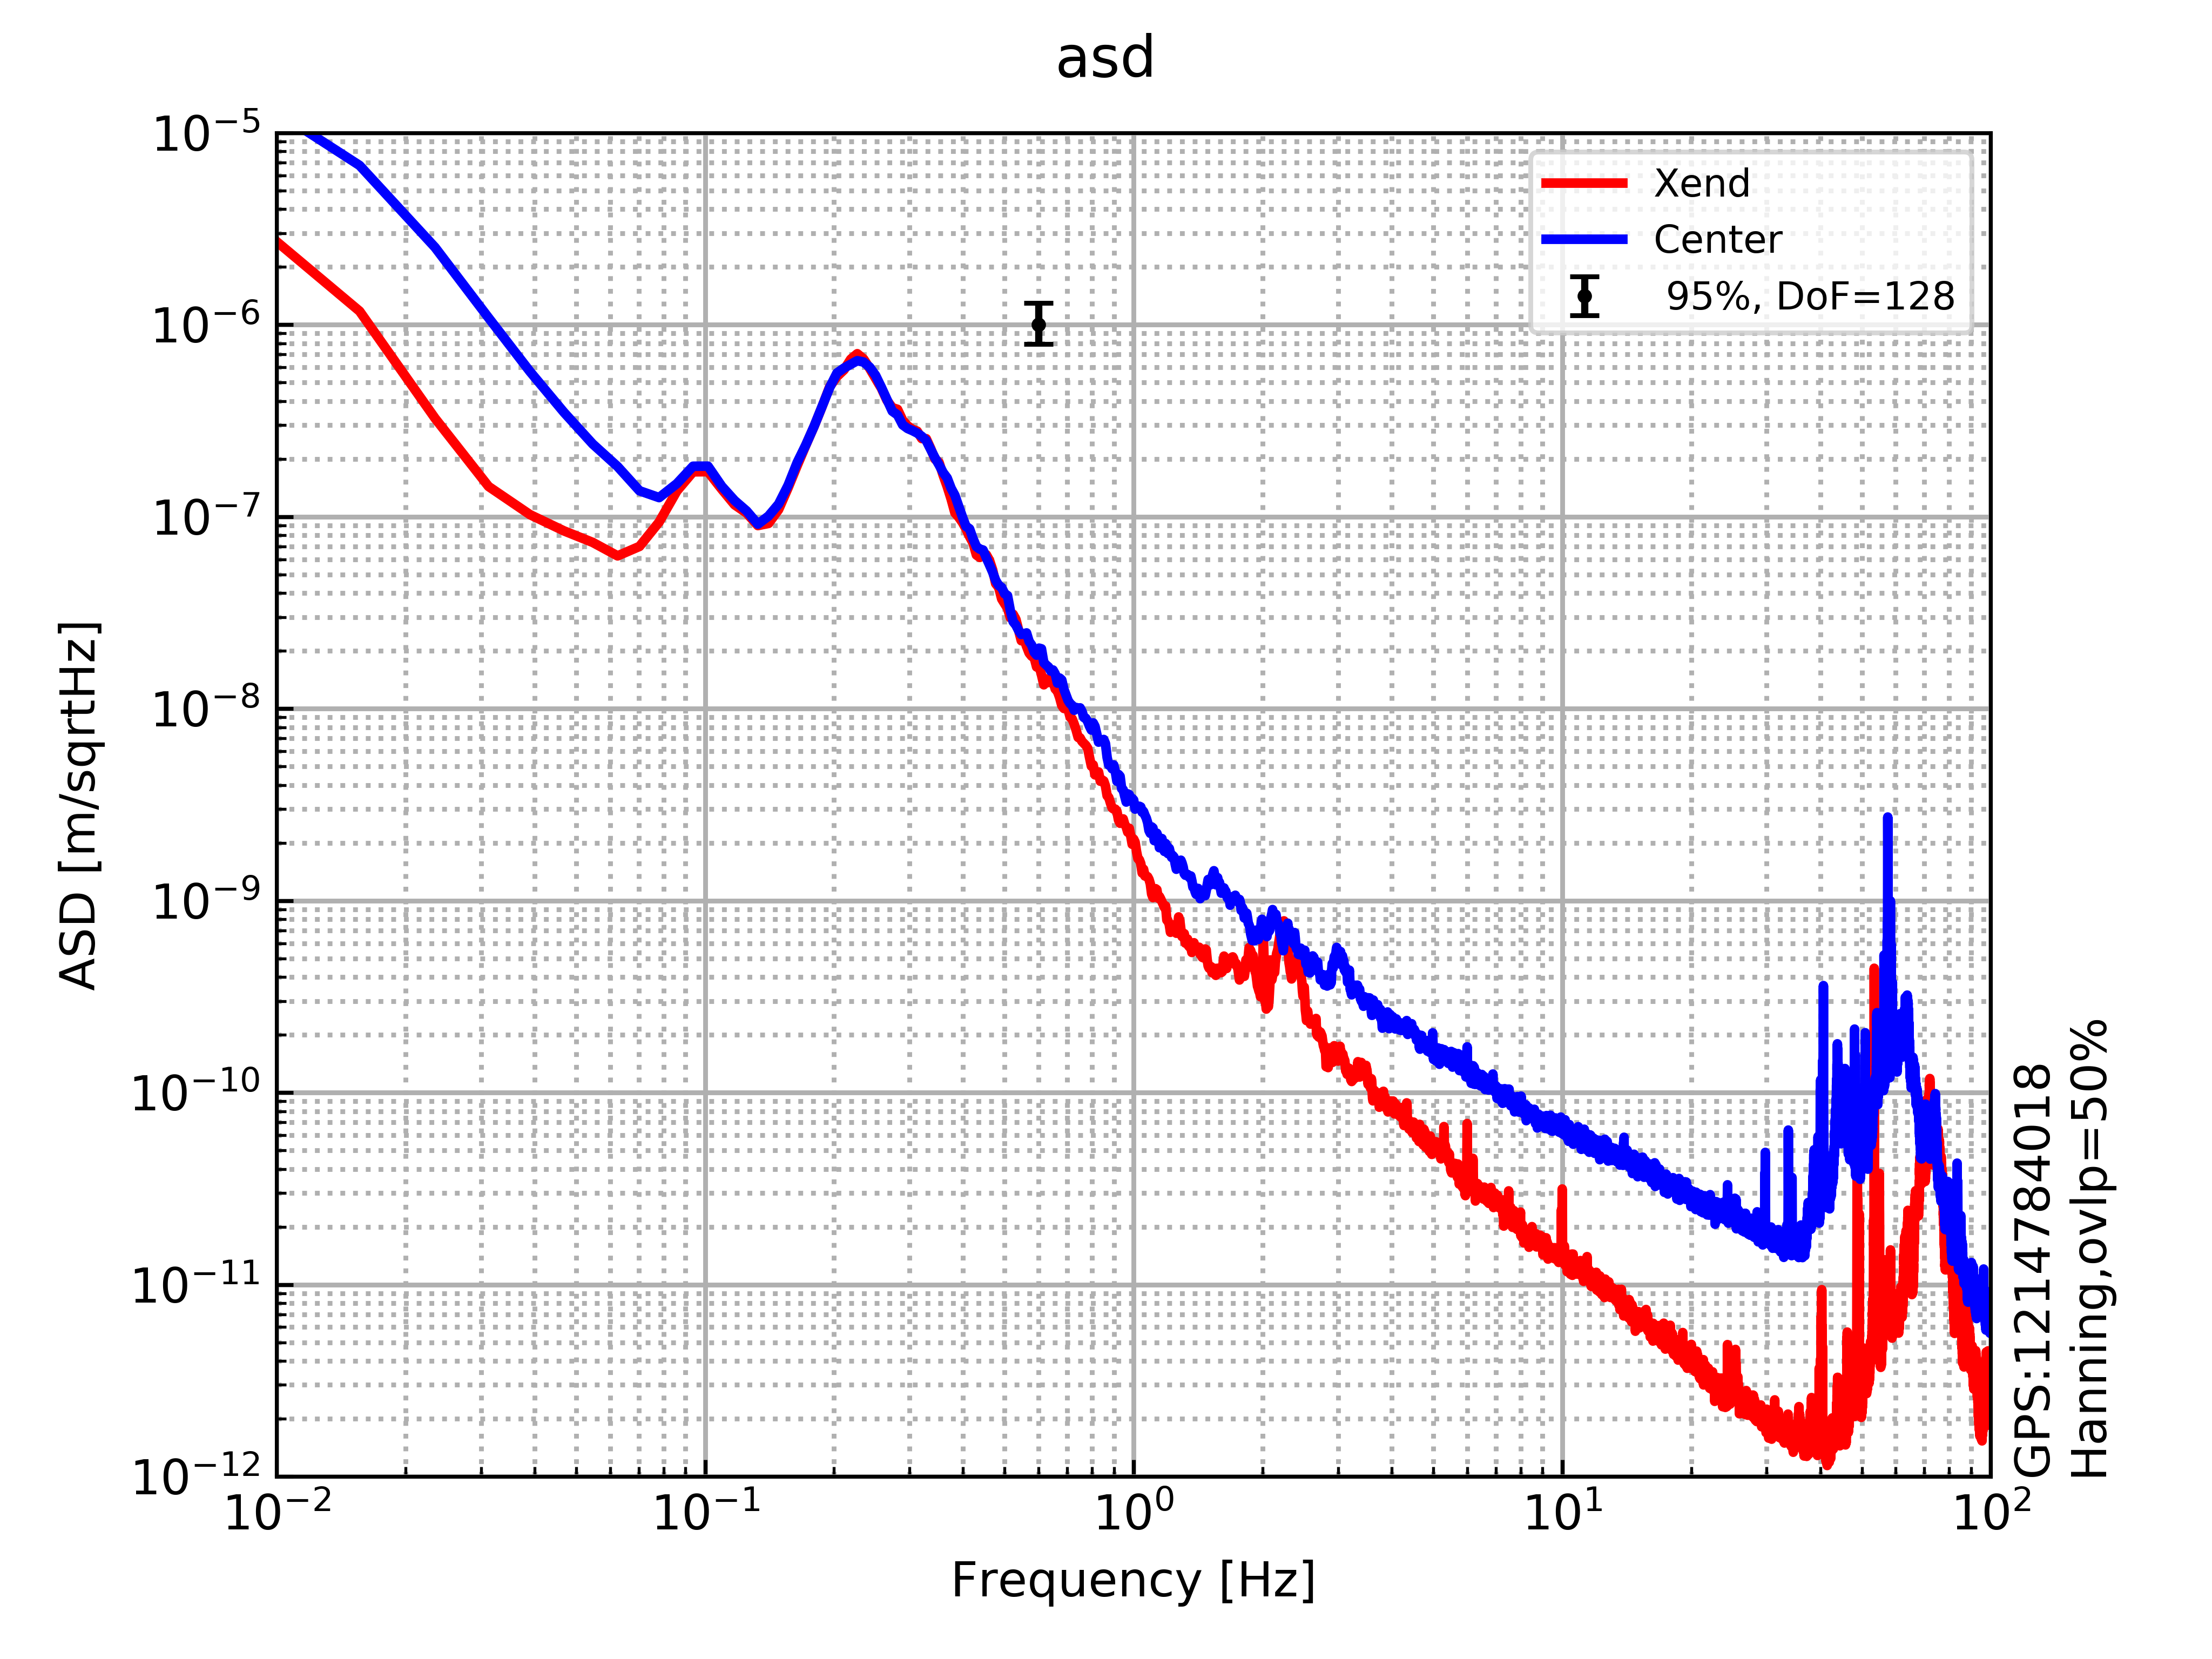
\includegraphics[width=11.5cm]{./img_asd_exvixv.png}
  \end{center}
  \caption{Xエンドとセンターエリアにおいた地震計のXアーム方向のASD。速度出力の地震計の信号を$2\pi{f}$で割って変位に換算している。エラーバーは95%の信頼区間。時系列データは2018/07/05 00:00:00 (JST)から$2^{13}$秒(2.3時間)分をつかった。平均回数は64回で,窓関数はHanning窓をつかった。}\label{img:img1}
\end{figure}


\subsubsection{地震計のコヒーレンス}
\begin{figure}[H]
  \begin{center}
    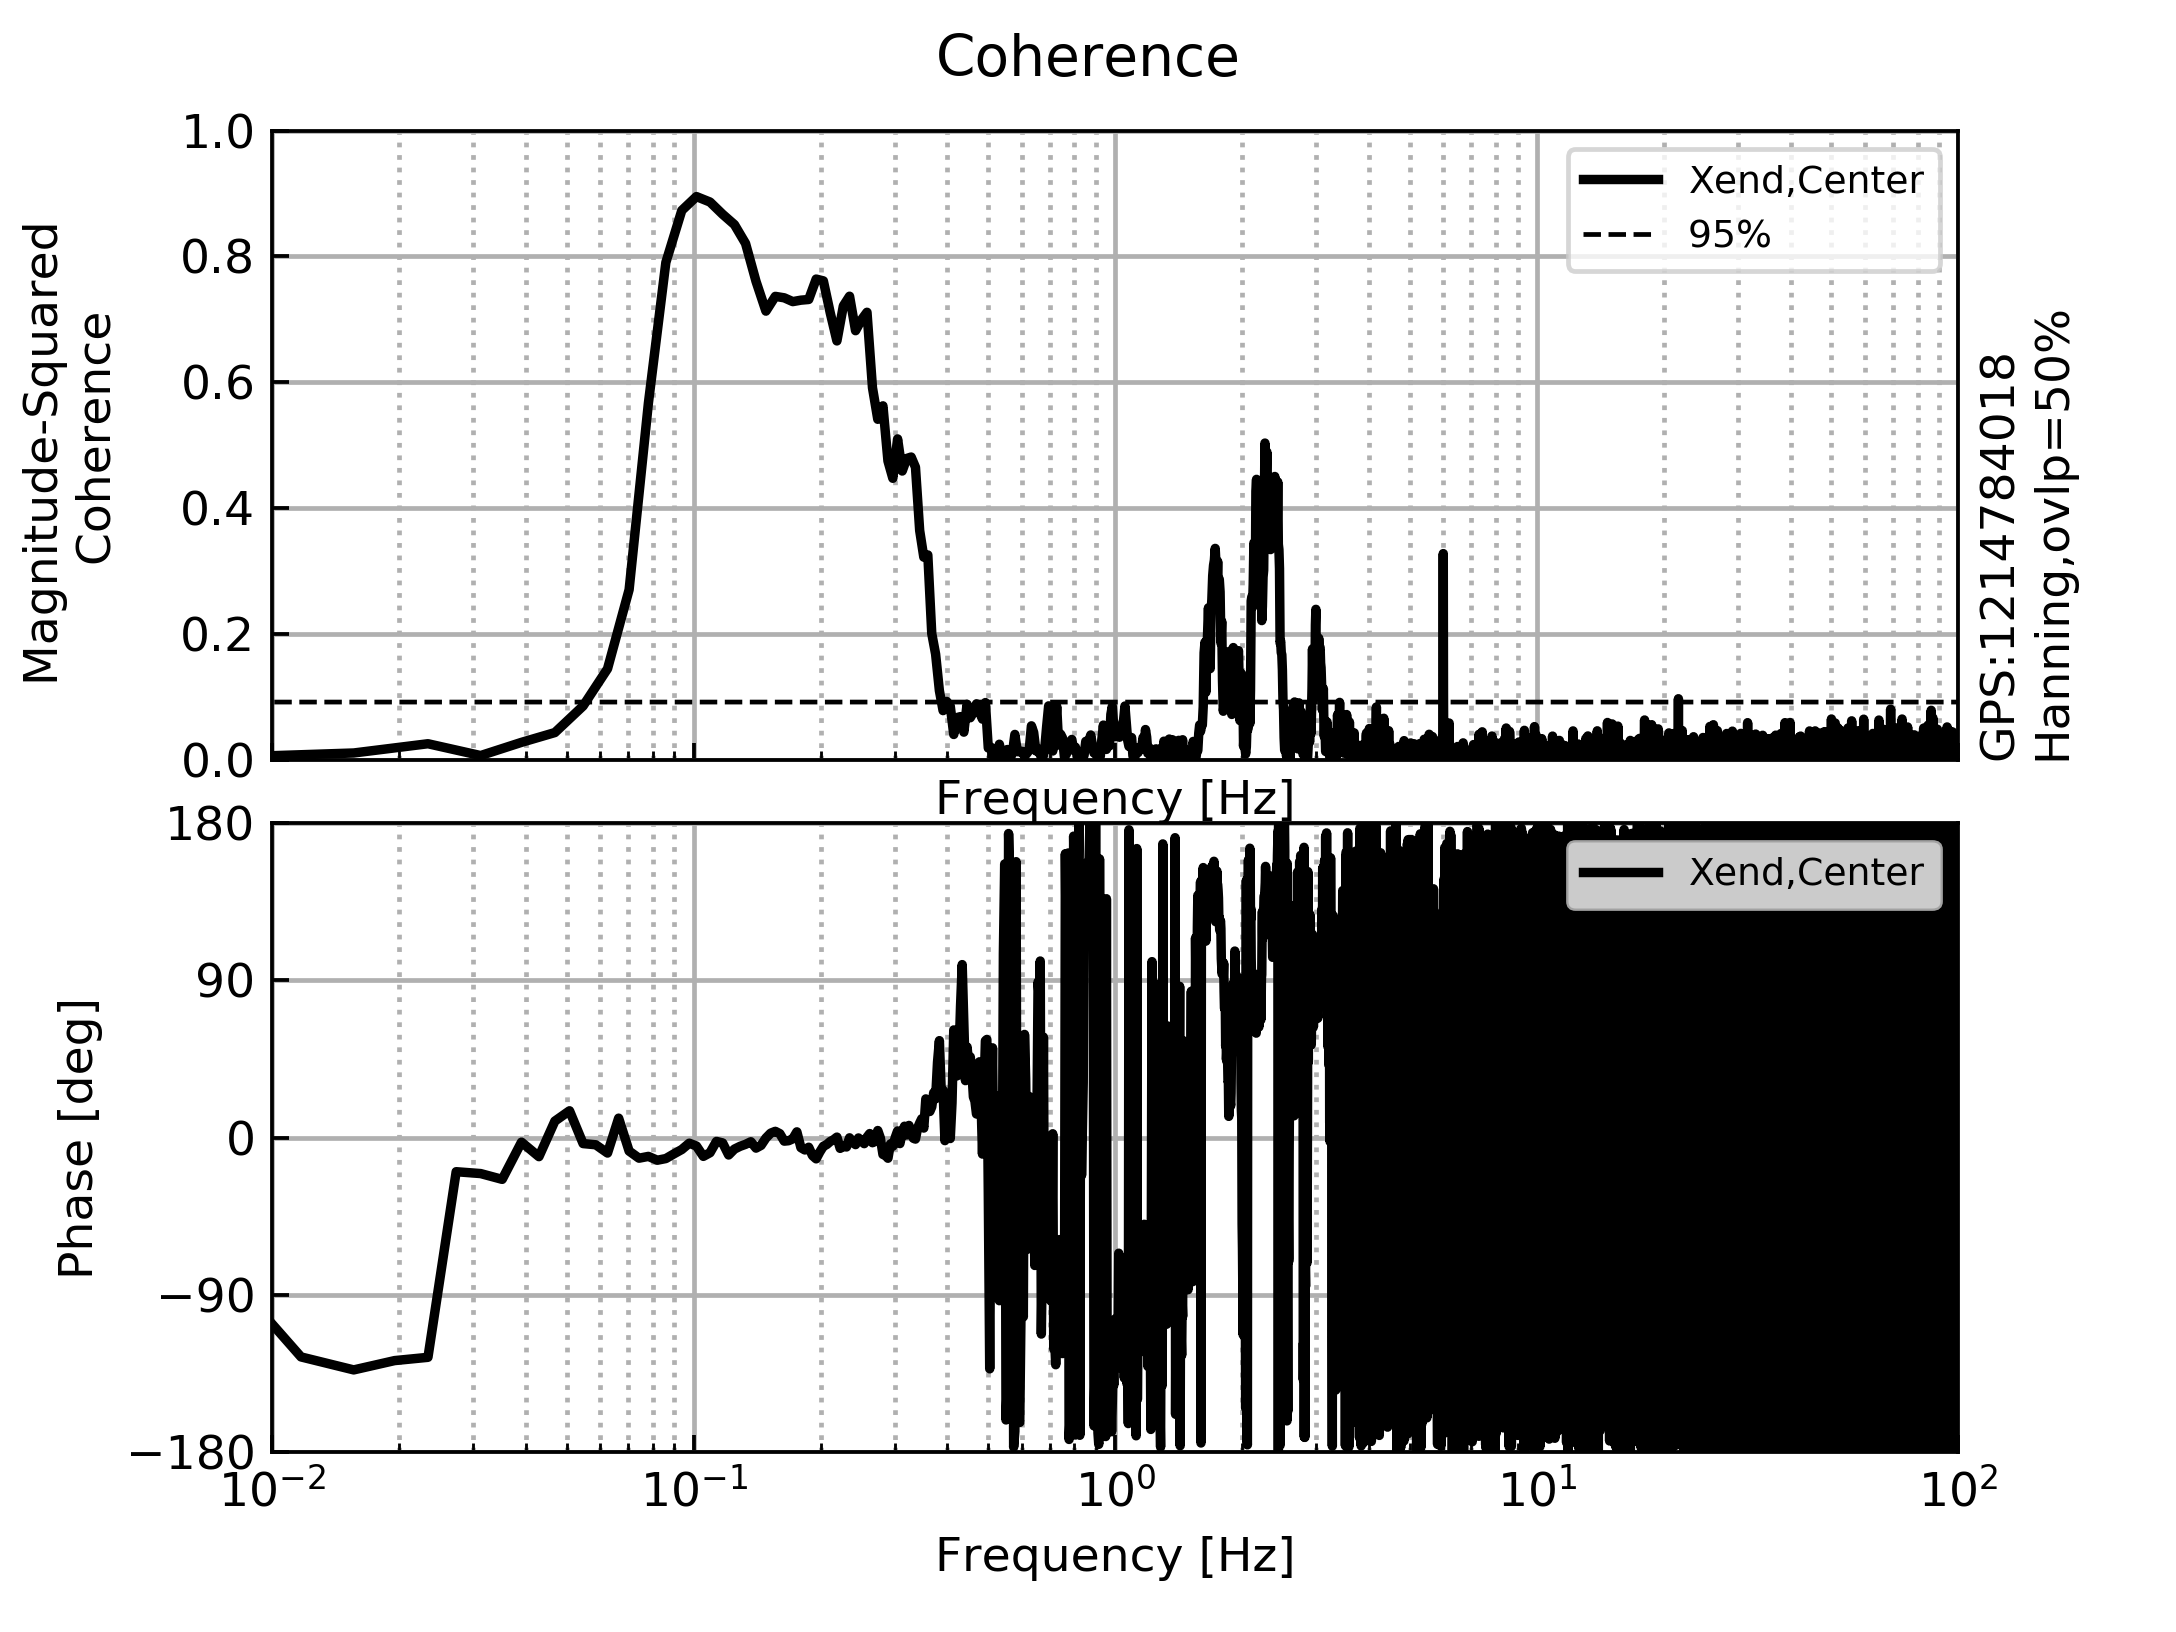
\includegraphics[width=11.5cm]{./img_coh_exvixv.png}
  \end{center}
  \caption{Xエンドとセンターエリアにおいた地震計のXアーム方向同士のコヒーレンス。破線より上にあれば,5%の有意水準でコヒーレンスがないという帰無仮説を棄却でき,コヒーレンスがあると言える。}\label{img:img2}
\end{figure}


図\ref{img:img2}に,Xエンドとセンターの地震計同士のコヒーレンスを示す。コヒーレンスは,0.1-0.3Hzと2Hz周辺で有意に存在する。前者の帯域では位相差は0度になっており同相成分が多いことが期待できる。これは脈動由来だと考えられるが,一方で後者の由来はまだわからない。\footnote[8]{いろんな時系列で同じ解析をしていないので,なんともいえないけれど,このピークはいつもは現れない。雨が多く降ったときにみえる。}低音懸架の1.6Hzの基線長方向の共振モードと被っているので,RMSを大きくしてしまうので注意が必要。


\subsubsection{$\mathrm{CDMR_{seis}}$}
\begin{figure}[H]
  \begin{center}
    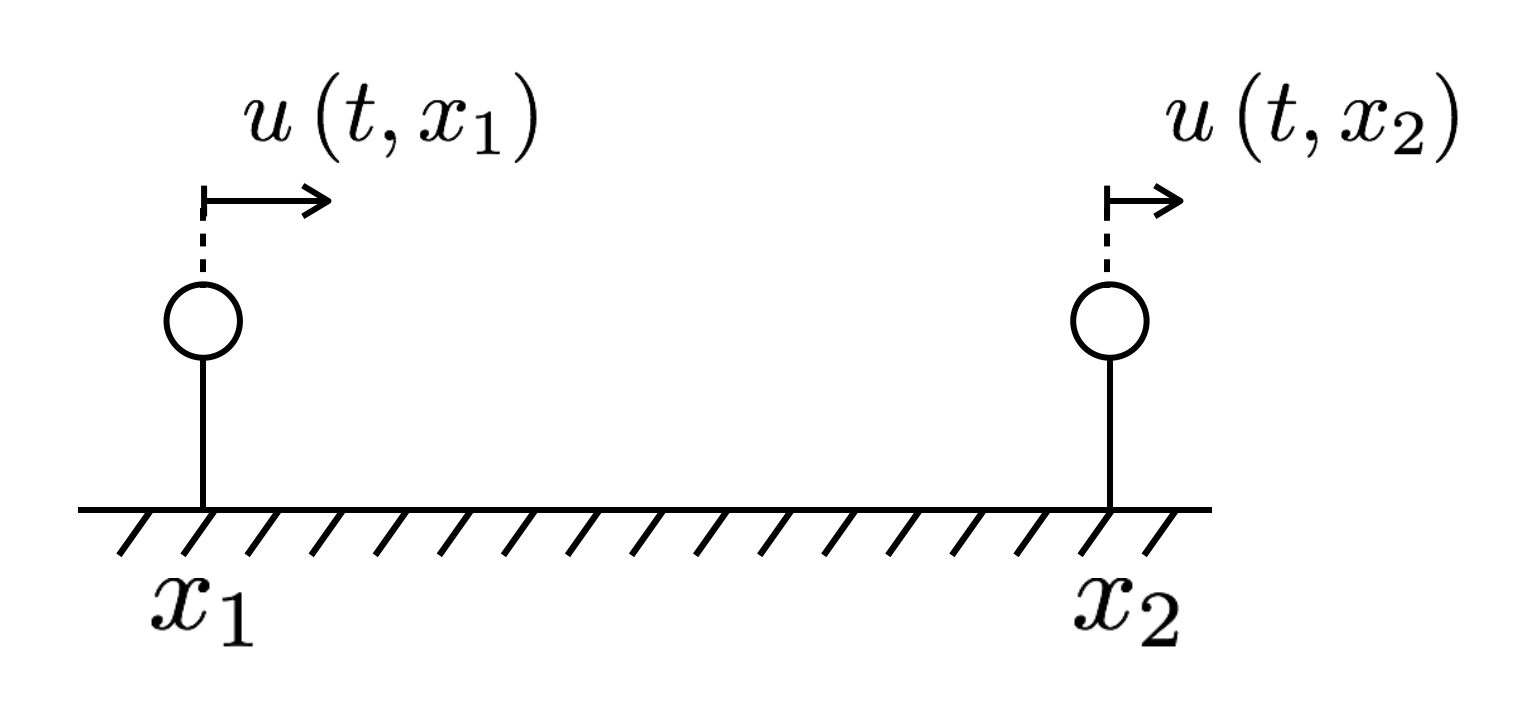
\includegraphics[width=11.5cm]{./img_cdmr_xarm.png}
  \end{center}
  \caption{上図:3km離れた二点の地面振動の同相成分と逆相成分のASD。0.1-0.2Hz付近にピークをもつ脈動では同相成分のほうが逆相成分よりも大きい。下図:同相成分と逆相成分の比(CDMR)。緑色の破線は,位相速度$5500\, \mathrm{m/s}$平面波がXアームを伝搬した場合のCDMRを示す。青色の破線は,相関がない場合のCMDRを示す。脈動はコヒーレンスがあり,波長はKAGRAの基線長よりも長いので,同相雑音が低減されている。}\label{img:img3}
\end{figure}


式\ref{eq:eq18}にP波の位相速度$5500\, \mathrm{m/s}$を代入した\footnote[9]{本来はレイリー波の速度が適している?}ものを図\ref{img:img3}の下図に緑色の破線で示す。この平面波のモデルと、実測データからもとめたCDMRを比較すると、コヒーレンスがある帯域で一致することがわかる。その他の帯域では,ADCノイズや傾斜ノイズによってコヒーレンスがなくなっているため,式\ref{eq:eq33}より,CDMRは1となる。(図\ref{img:img3}下図の青色破線)。\footnote[10]{思いの外,平面波のモデルと実測したものが一致している。他の期間でも同じ解析してみて,どうなるか気になる。}

\subsubsection{$\mathrm{CDMR_{gif}}$}
\begin{figure}[H]
  \begin{center}
    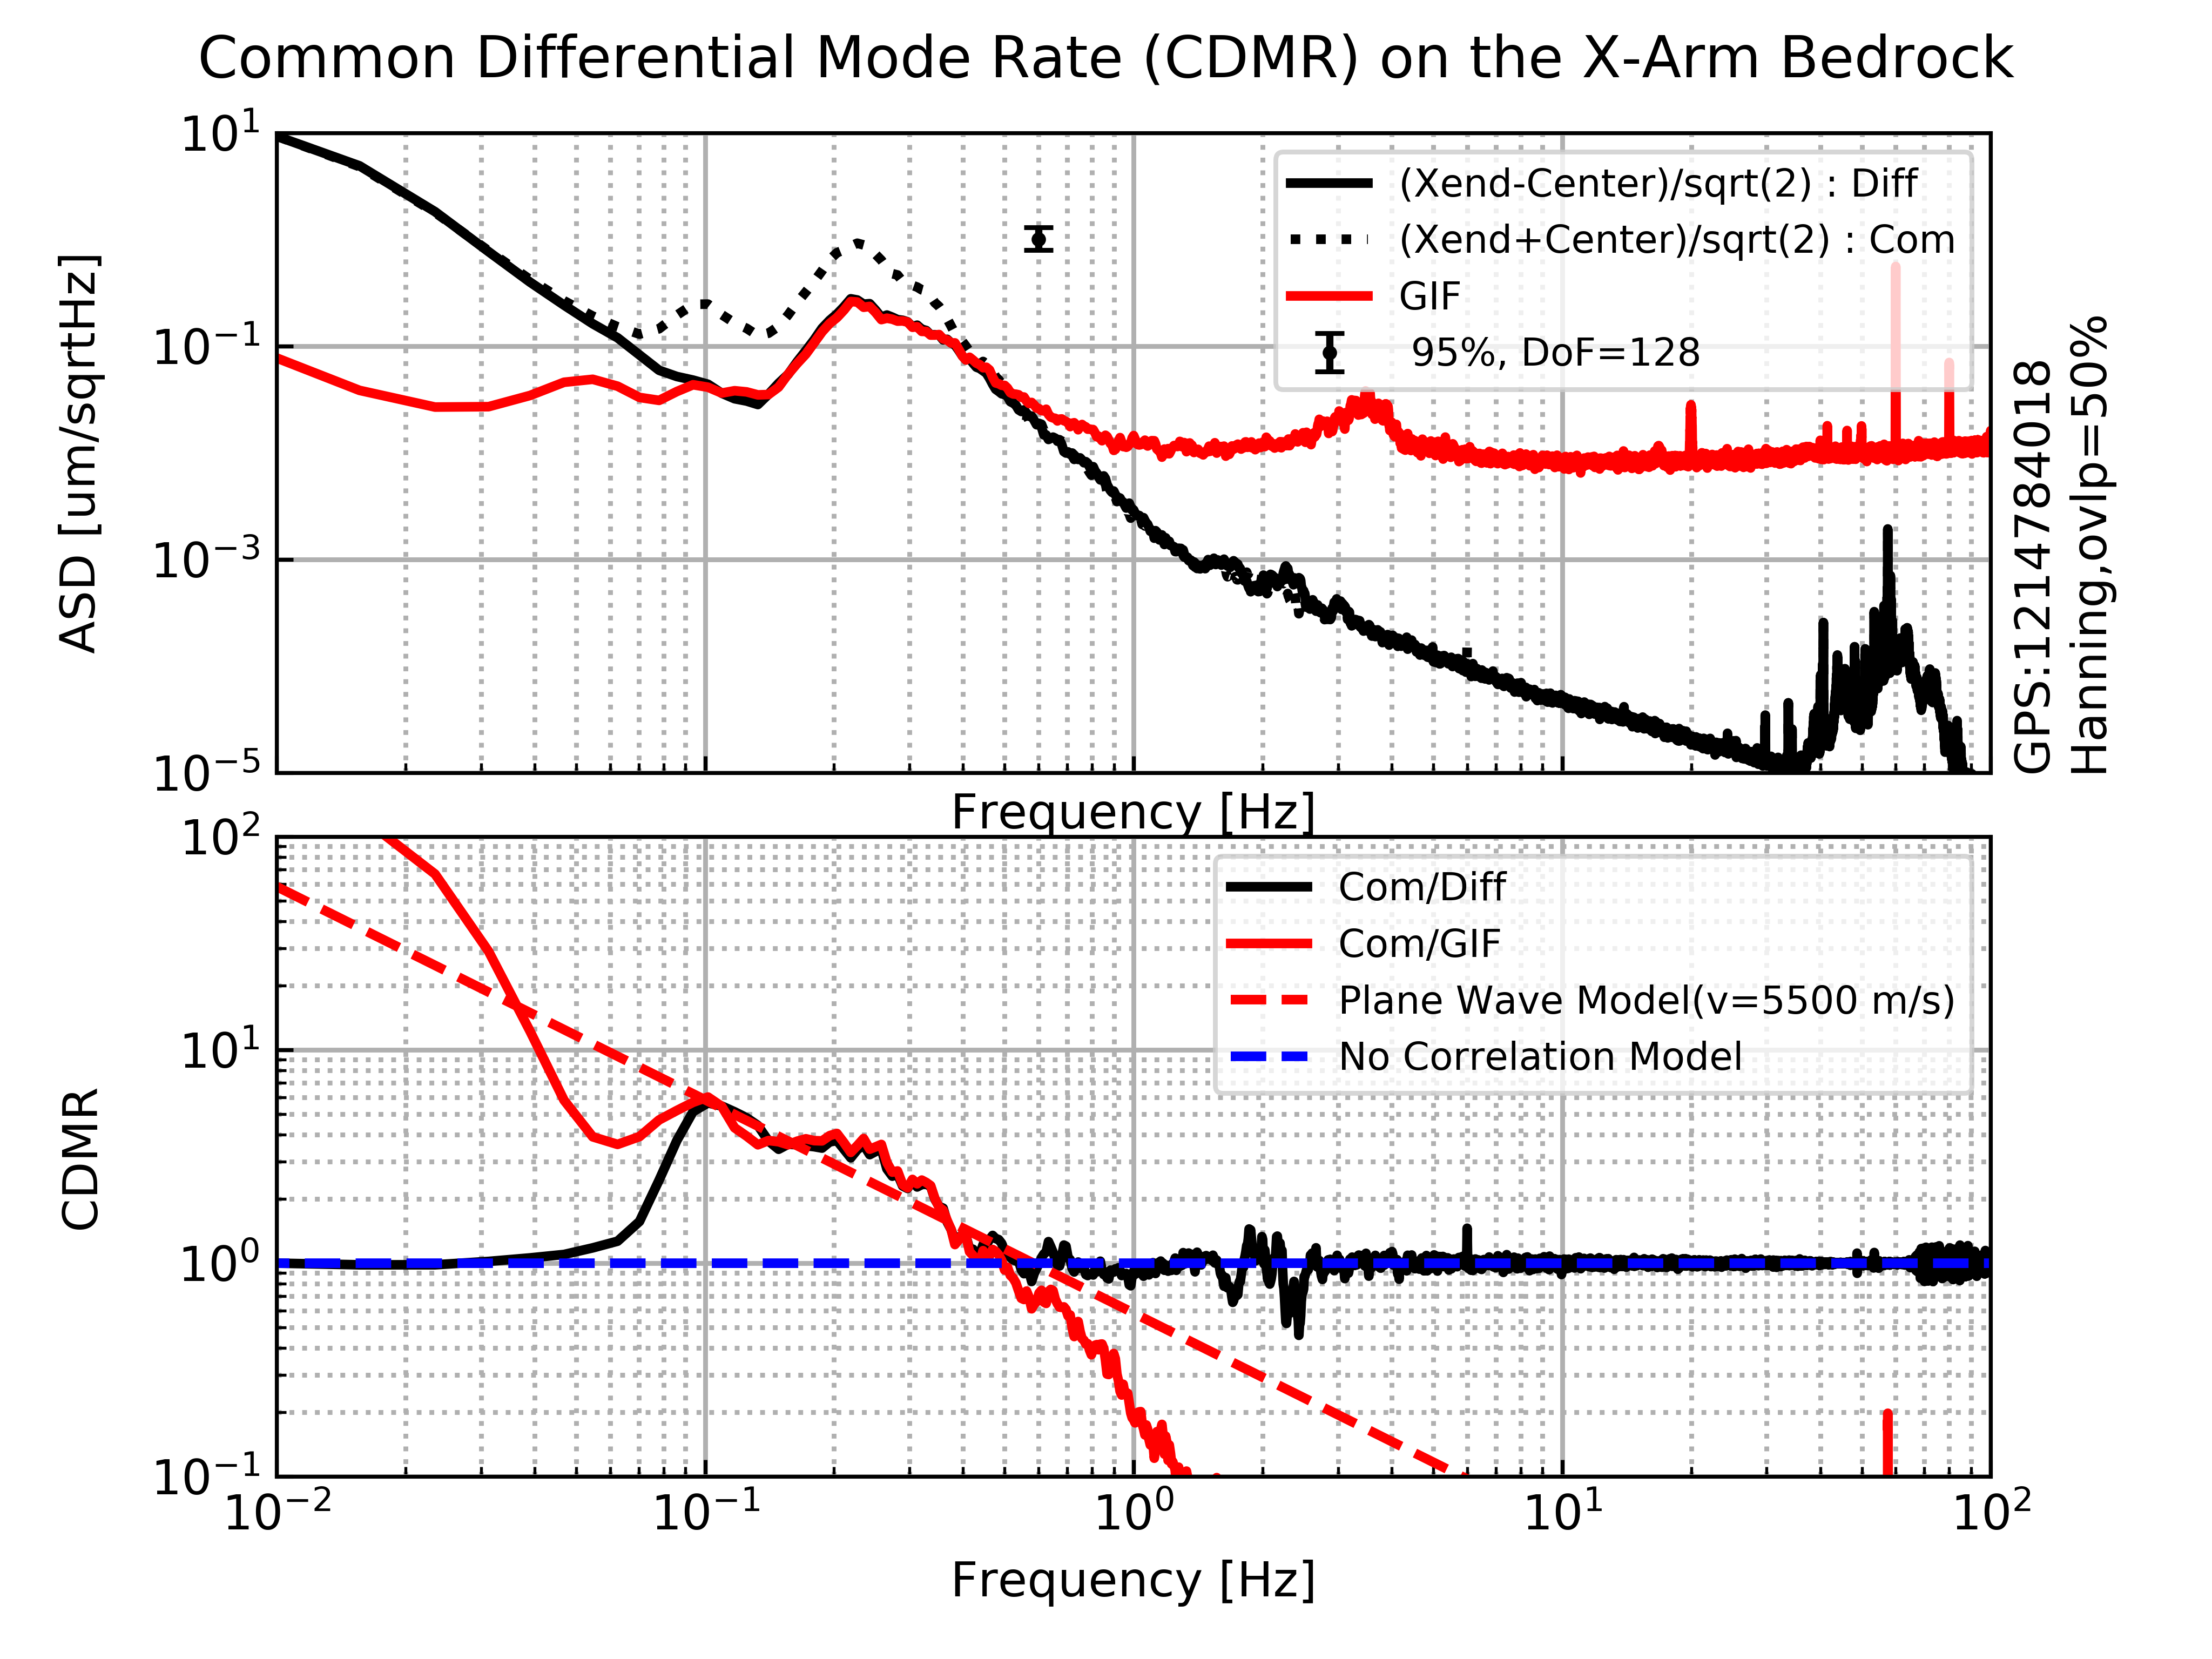
\includegraphics[width=11.5cm]{./img_cdmr_xarm_gif.png}
  \end{center}
  \caption{図\ref{img:img3}にGIFで推定した逆相成分を加えて比較。上図:変位のASD。下図:逆相成分をGIFに置き換えた$\mathrm{CDMR_{gif}}$を赤線でプロット。
  }\label{img:img4}
\end{figure}


図\ref{img:img2}に,3000mの2点における逆相成分をGIFのひずみ信号から換算したものを赤線でプロットしたものを,図\ref{img:img3}に示す。図\ref{img:img3}上図のASDをみると,GIFと地震計は脈動の帯域ではよく一致している。高周波側は,GIFは周波数ノイズで埋もれている。低周波側はGIFのほうが小さいが,これは地震計が傾きのカップリング成分で埋もれているためと考えられる。原理的にはGIFは,傾き成分から基線長伸縮へのカップリングはないため,地震計とくらべて,脈動以下ではGIFは低ノイズな基線長伸縮モニターとなることがわかる。\footnote[11]{これが,自分のオリジナリティを支える部分になると思う。}

式(\ref{eq:eq39})の位相速度に花崗岩の弾性波速度である5500m/sを代入して図\ref{img:img3}の下図に赤色の破線で示す。地震計と同様に脈動の帯域では平面波のモデルと一致する。


\subsection{IMCのCDMR}
IMCのCDMRを求める。%図\ref{img:img_imcseis}のように,
MCiとMCerrreにTrilliumCompactを置き,基線長方向の信号をつかってCDMRをもとめた。


\subsubsection{地震計のスペクトル}

\begin{figure}[H]
  \begin{center}
    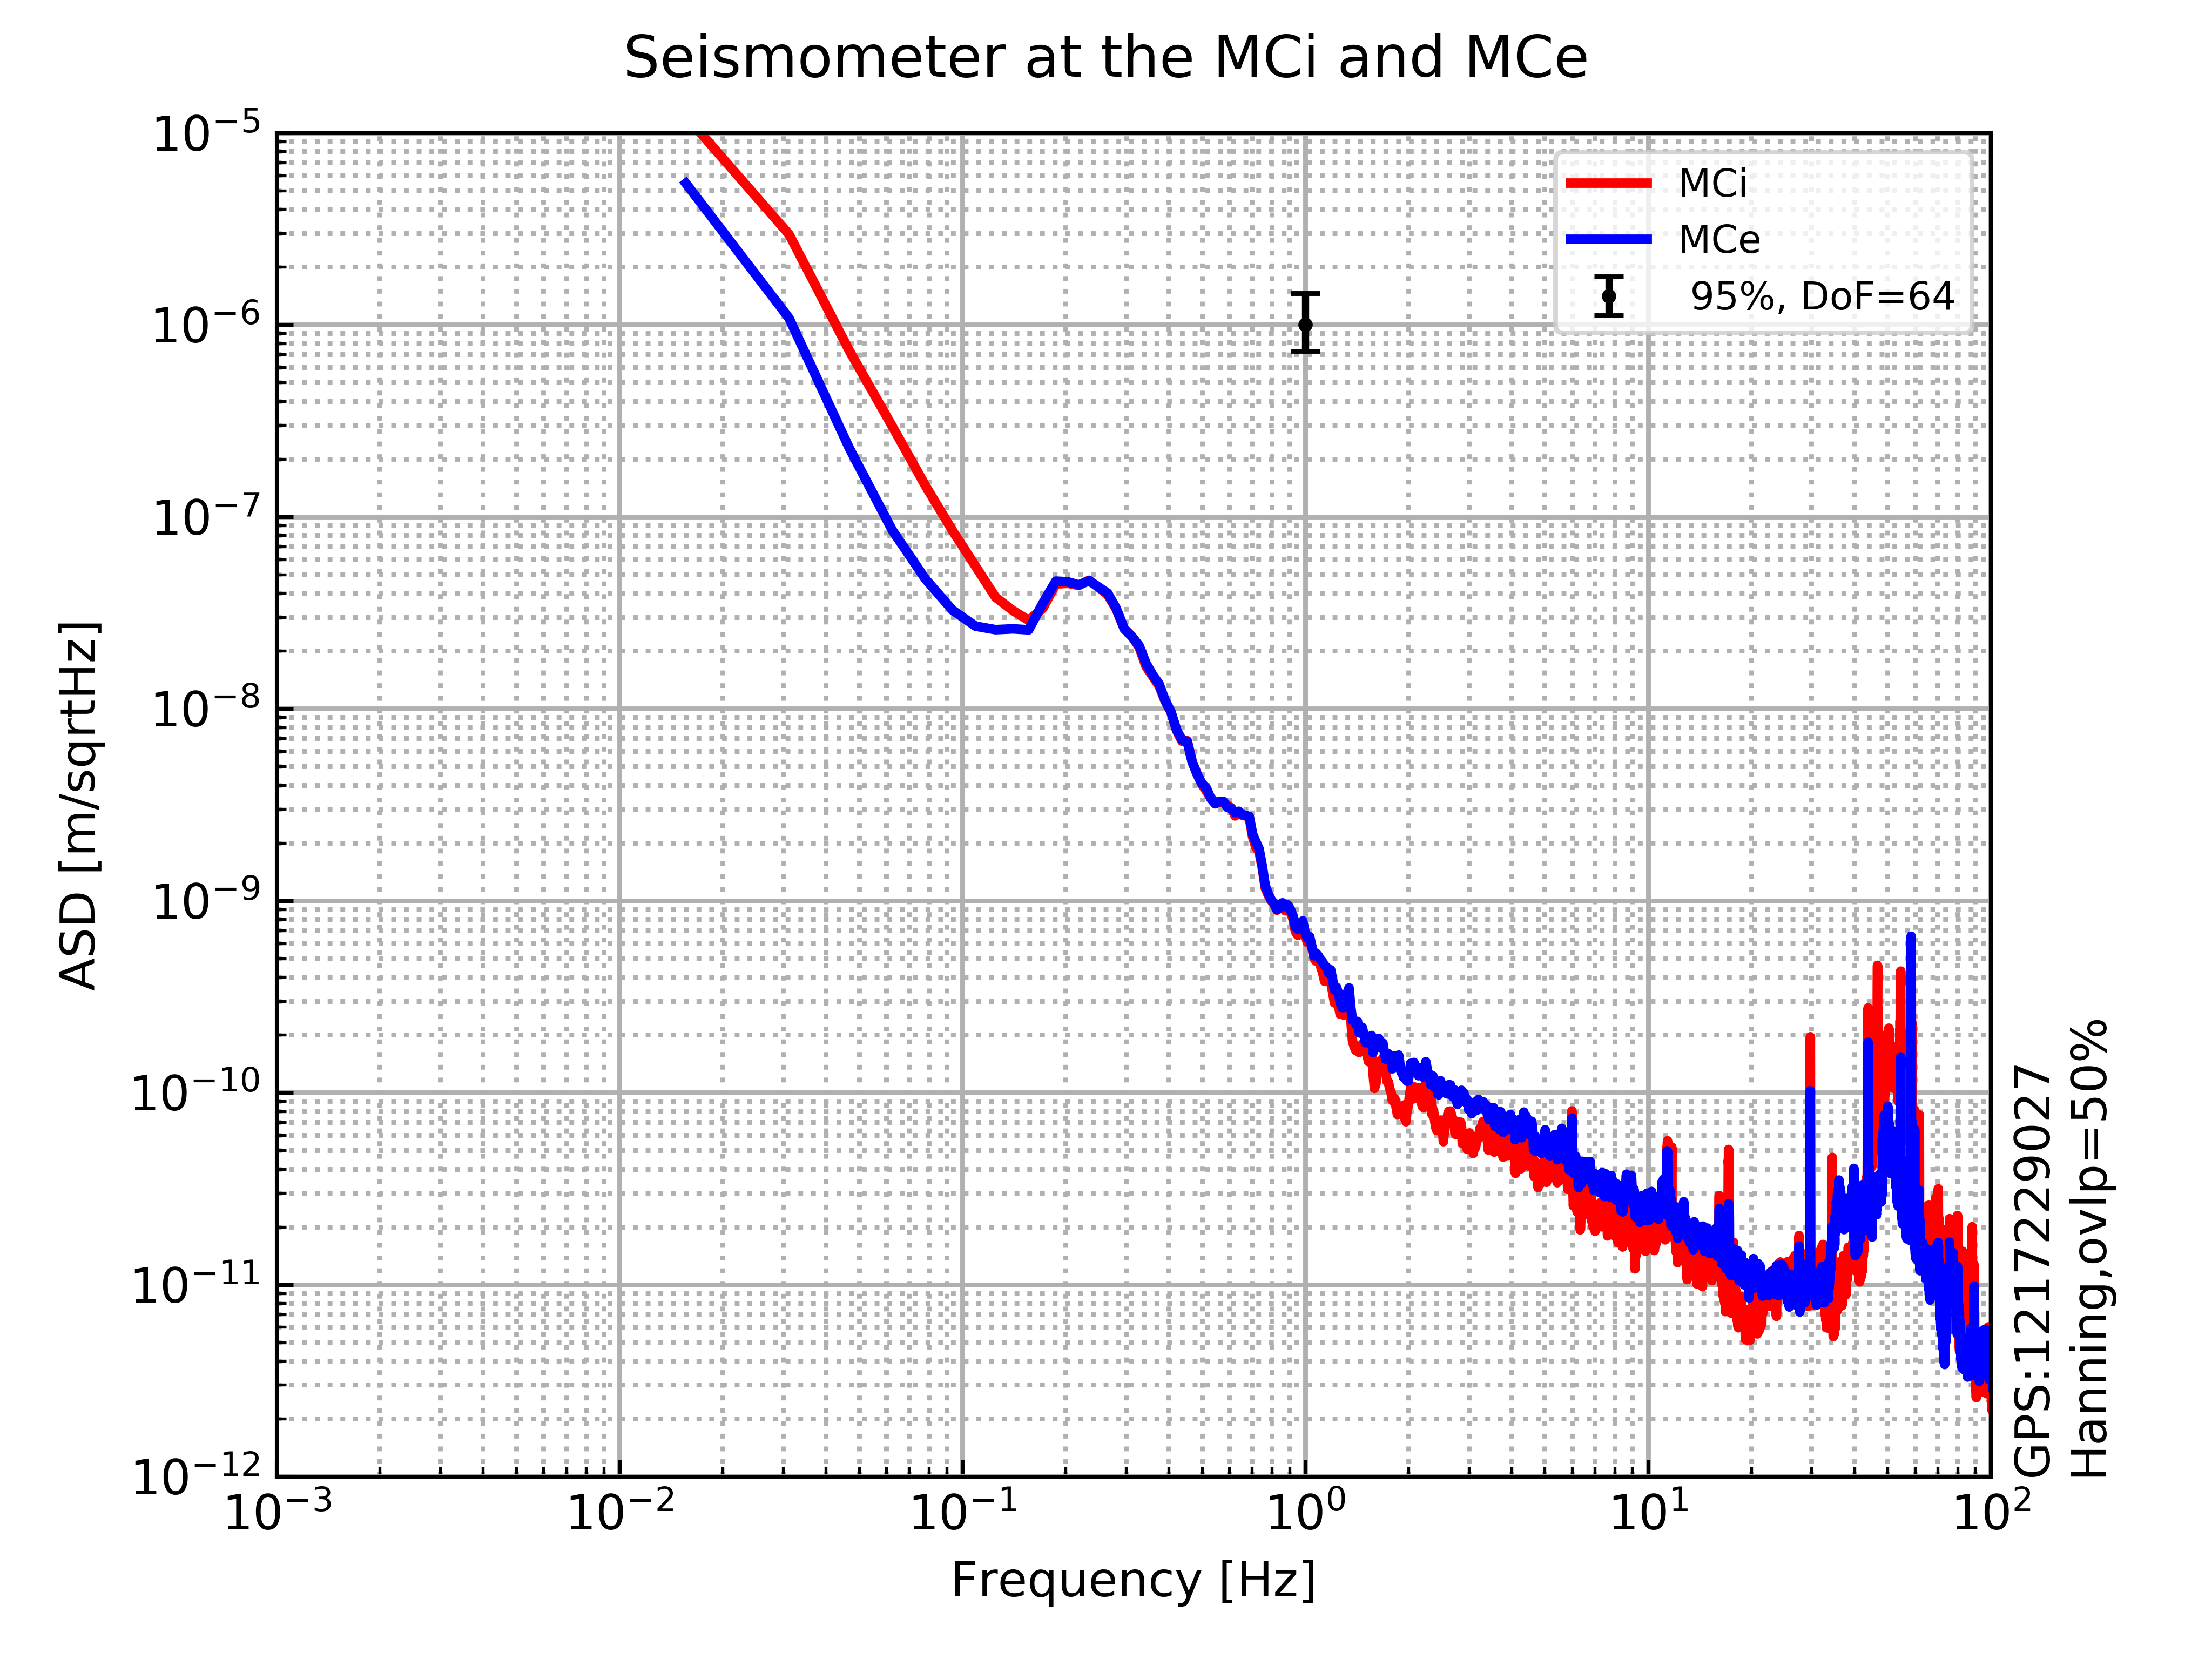
\includegraphics[width=11.5cm]{./img_asd_mcimce.png}
  \end{center}
  \caption{MCiとMCerrreのASD。時系列データは2018/08/02 07:10:09 (JST)から$2^{13}$秒(2.3時間)分をつかった。平均回数は64回で,窓関数はHanning窓をつかった。}\label{img:img_asd_imc}
\end{figure}

図\ref{img:img_asd_imc}にMCiとMCerrreにおいた地震計のASDを示す。エラーバーは95%の信頼区間を示す。0.2Hzから1Hzで2点は同じ地面振動レベルを示している。1-10Hzの帯域では,それぞれADCノイズに埋もれている。MCiの地震計は33倍のアンプを入れているのでADCノイズの換算雑音は小さい。


\subsubsection{地震計のコヒーレンス}

\begin{figure}[H]
  \begin{center}
    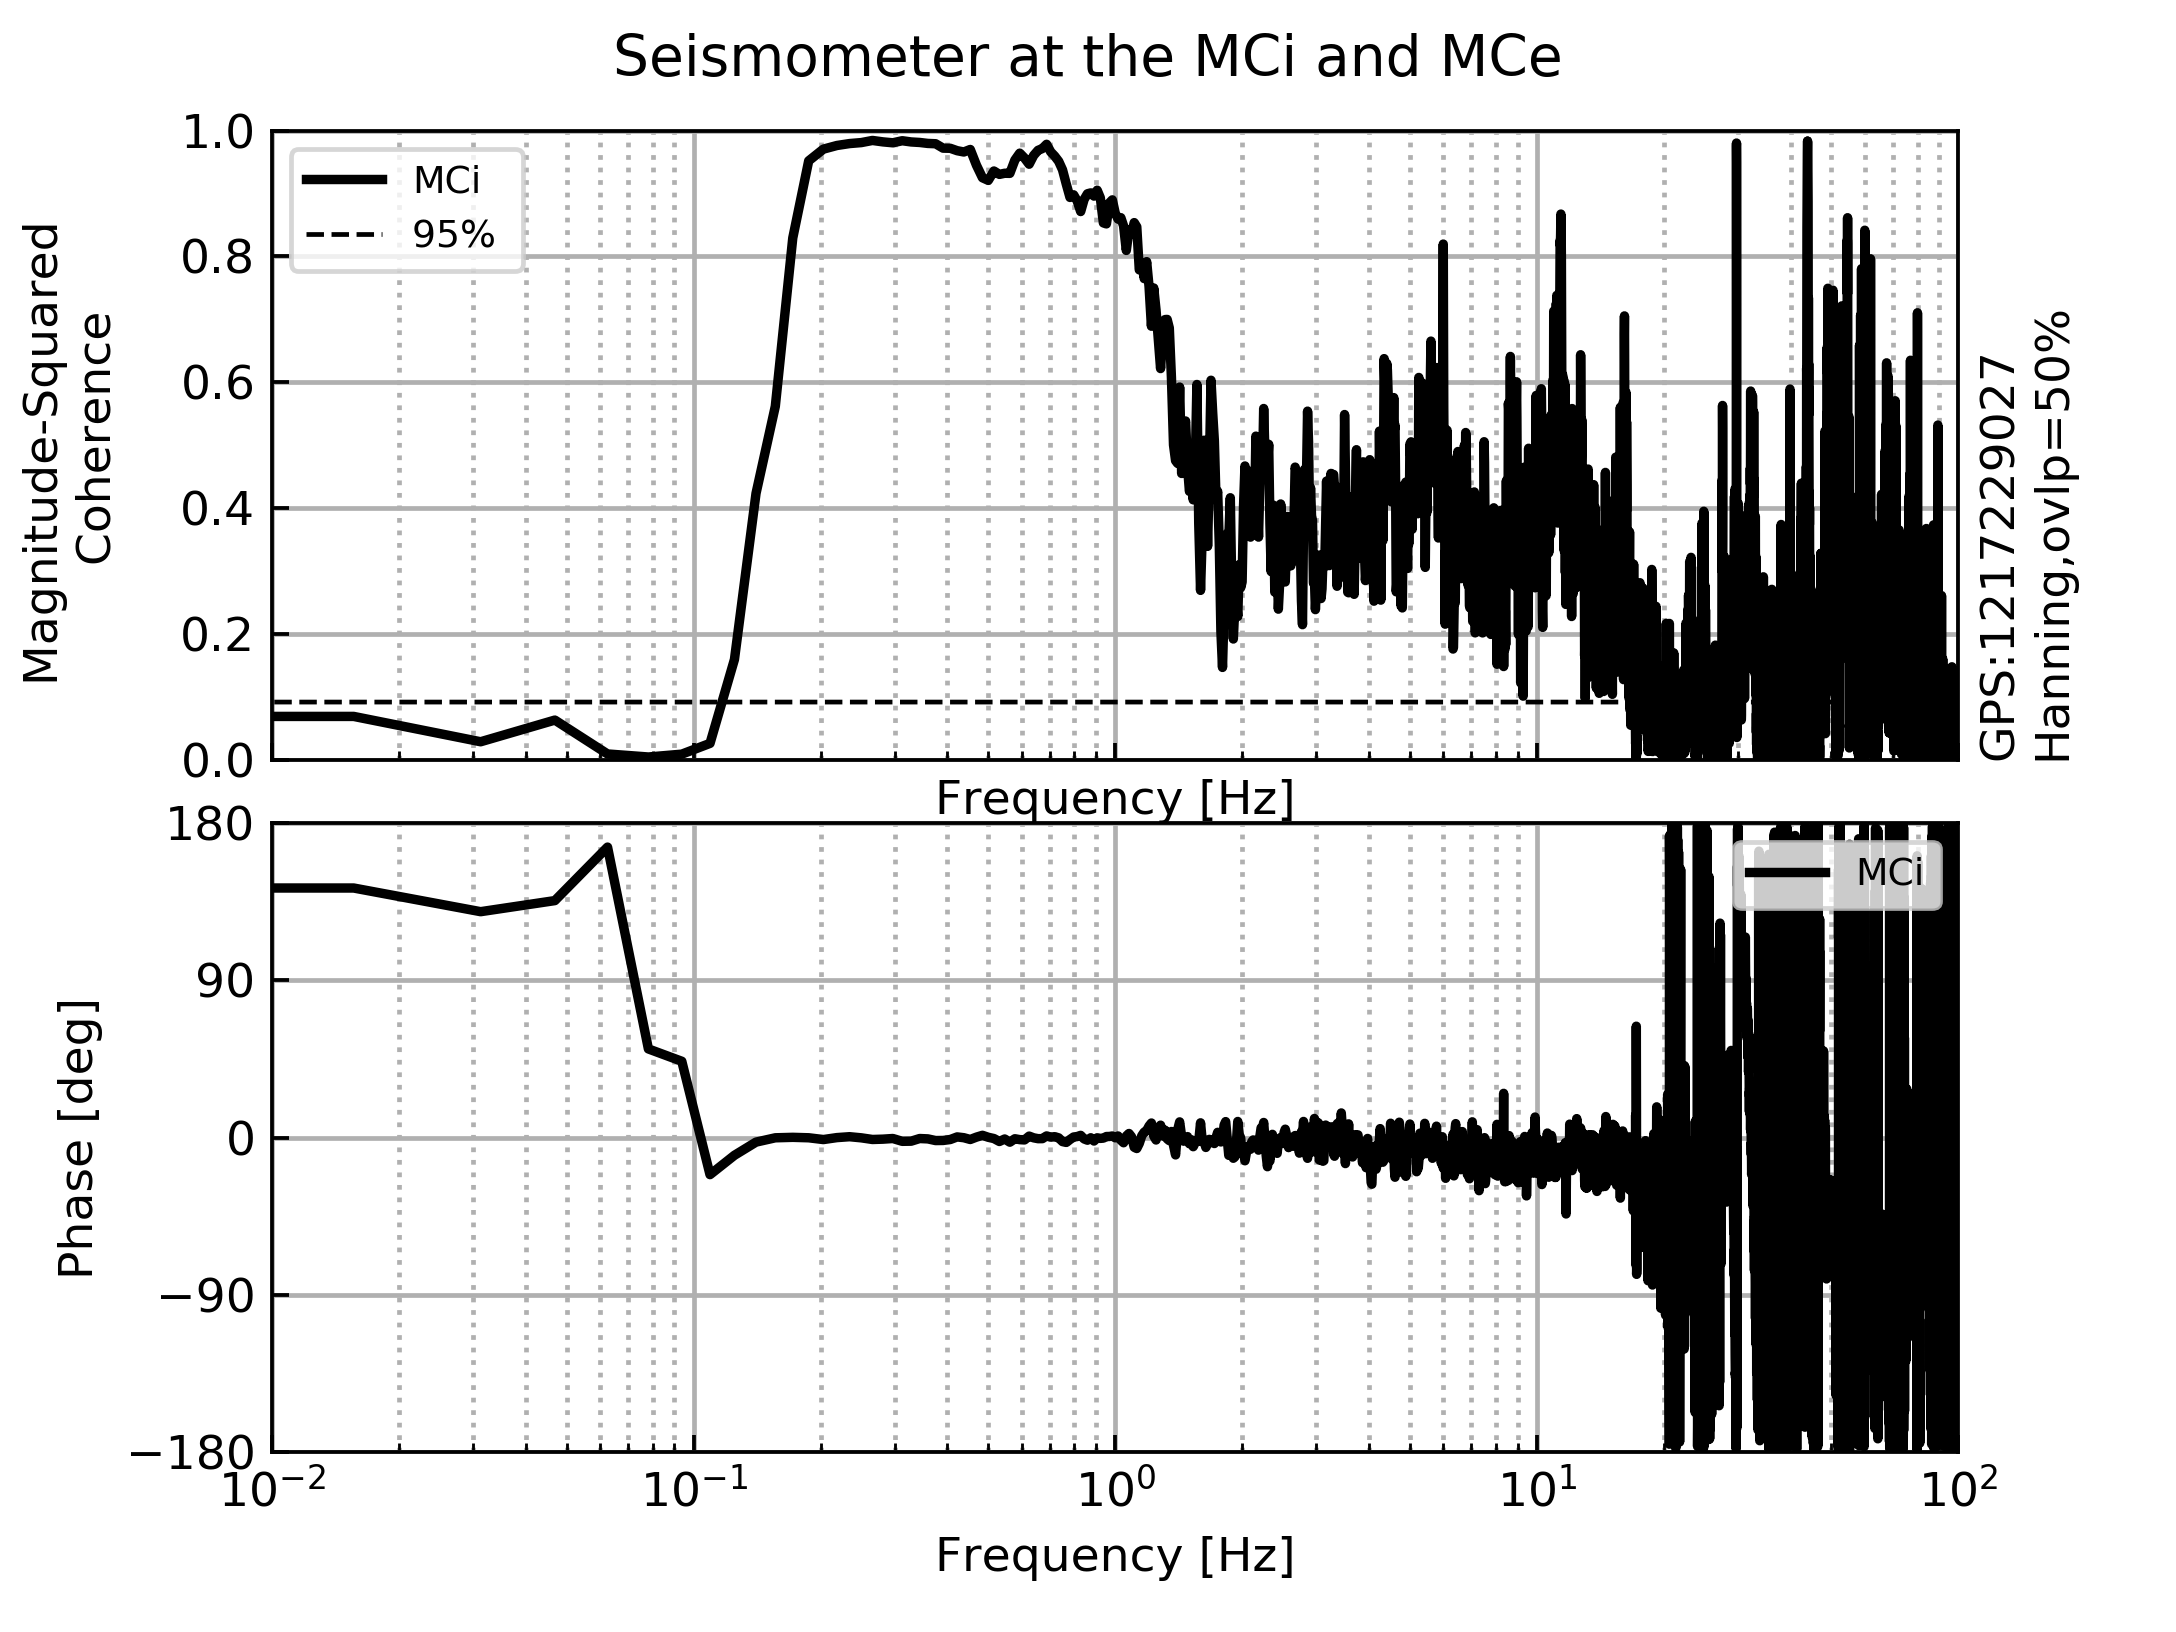
\includegraphics[width=11.5cm]{./img_coh_mcimce.png}
  \end{center}
  \caption{MCiとMCerrreのコヒーレンス。}\label{img:img_coherence_imc}
\end{figure}

図\ref{img:img_coherence_imc}にMCiとMCerrreのコヒーレンスを示す。0.2Hzから10Hzまで有意にコヒーレンスをもっている。とくに0.2−1Hzの帯域では非常にコヒーレンスが高い。また位相差が0となっているため,2点は同相で動いていることがわかる。



\subsubsection{$\mathrm{CDMR_{seis}}$}
\begin{figure}[H]
  \begin{center}
    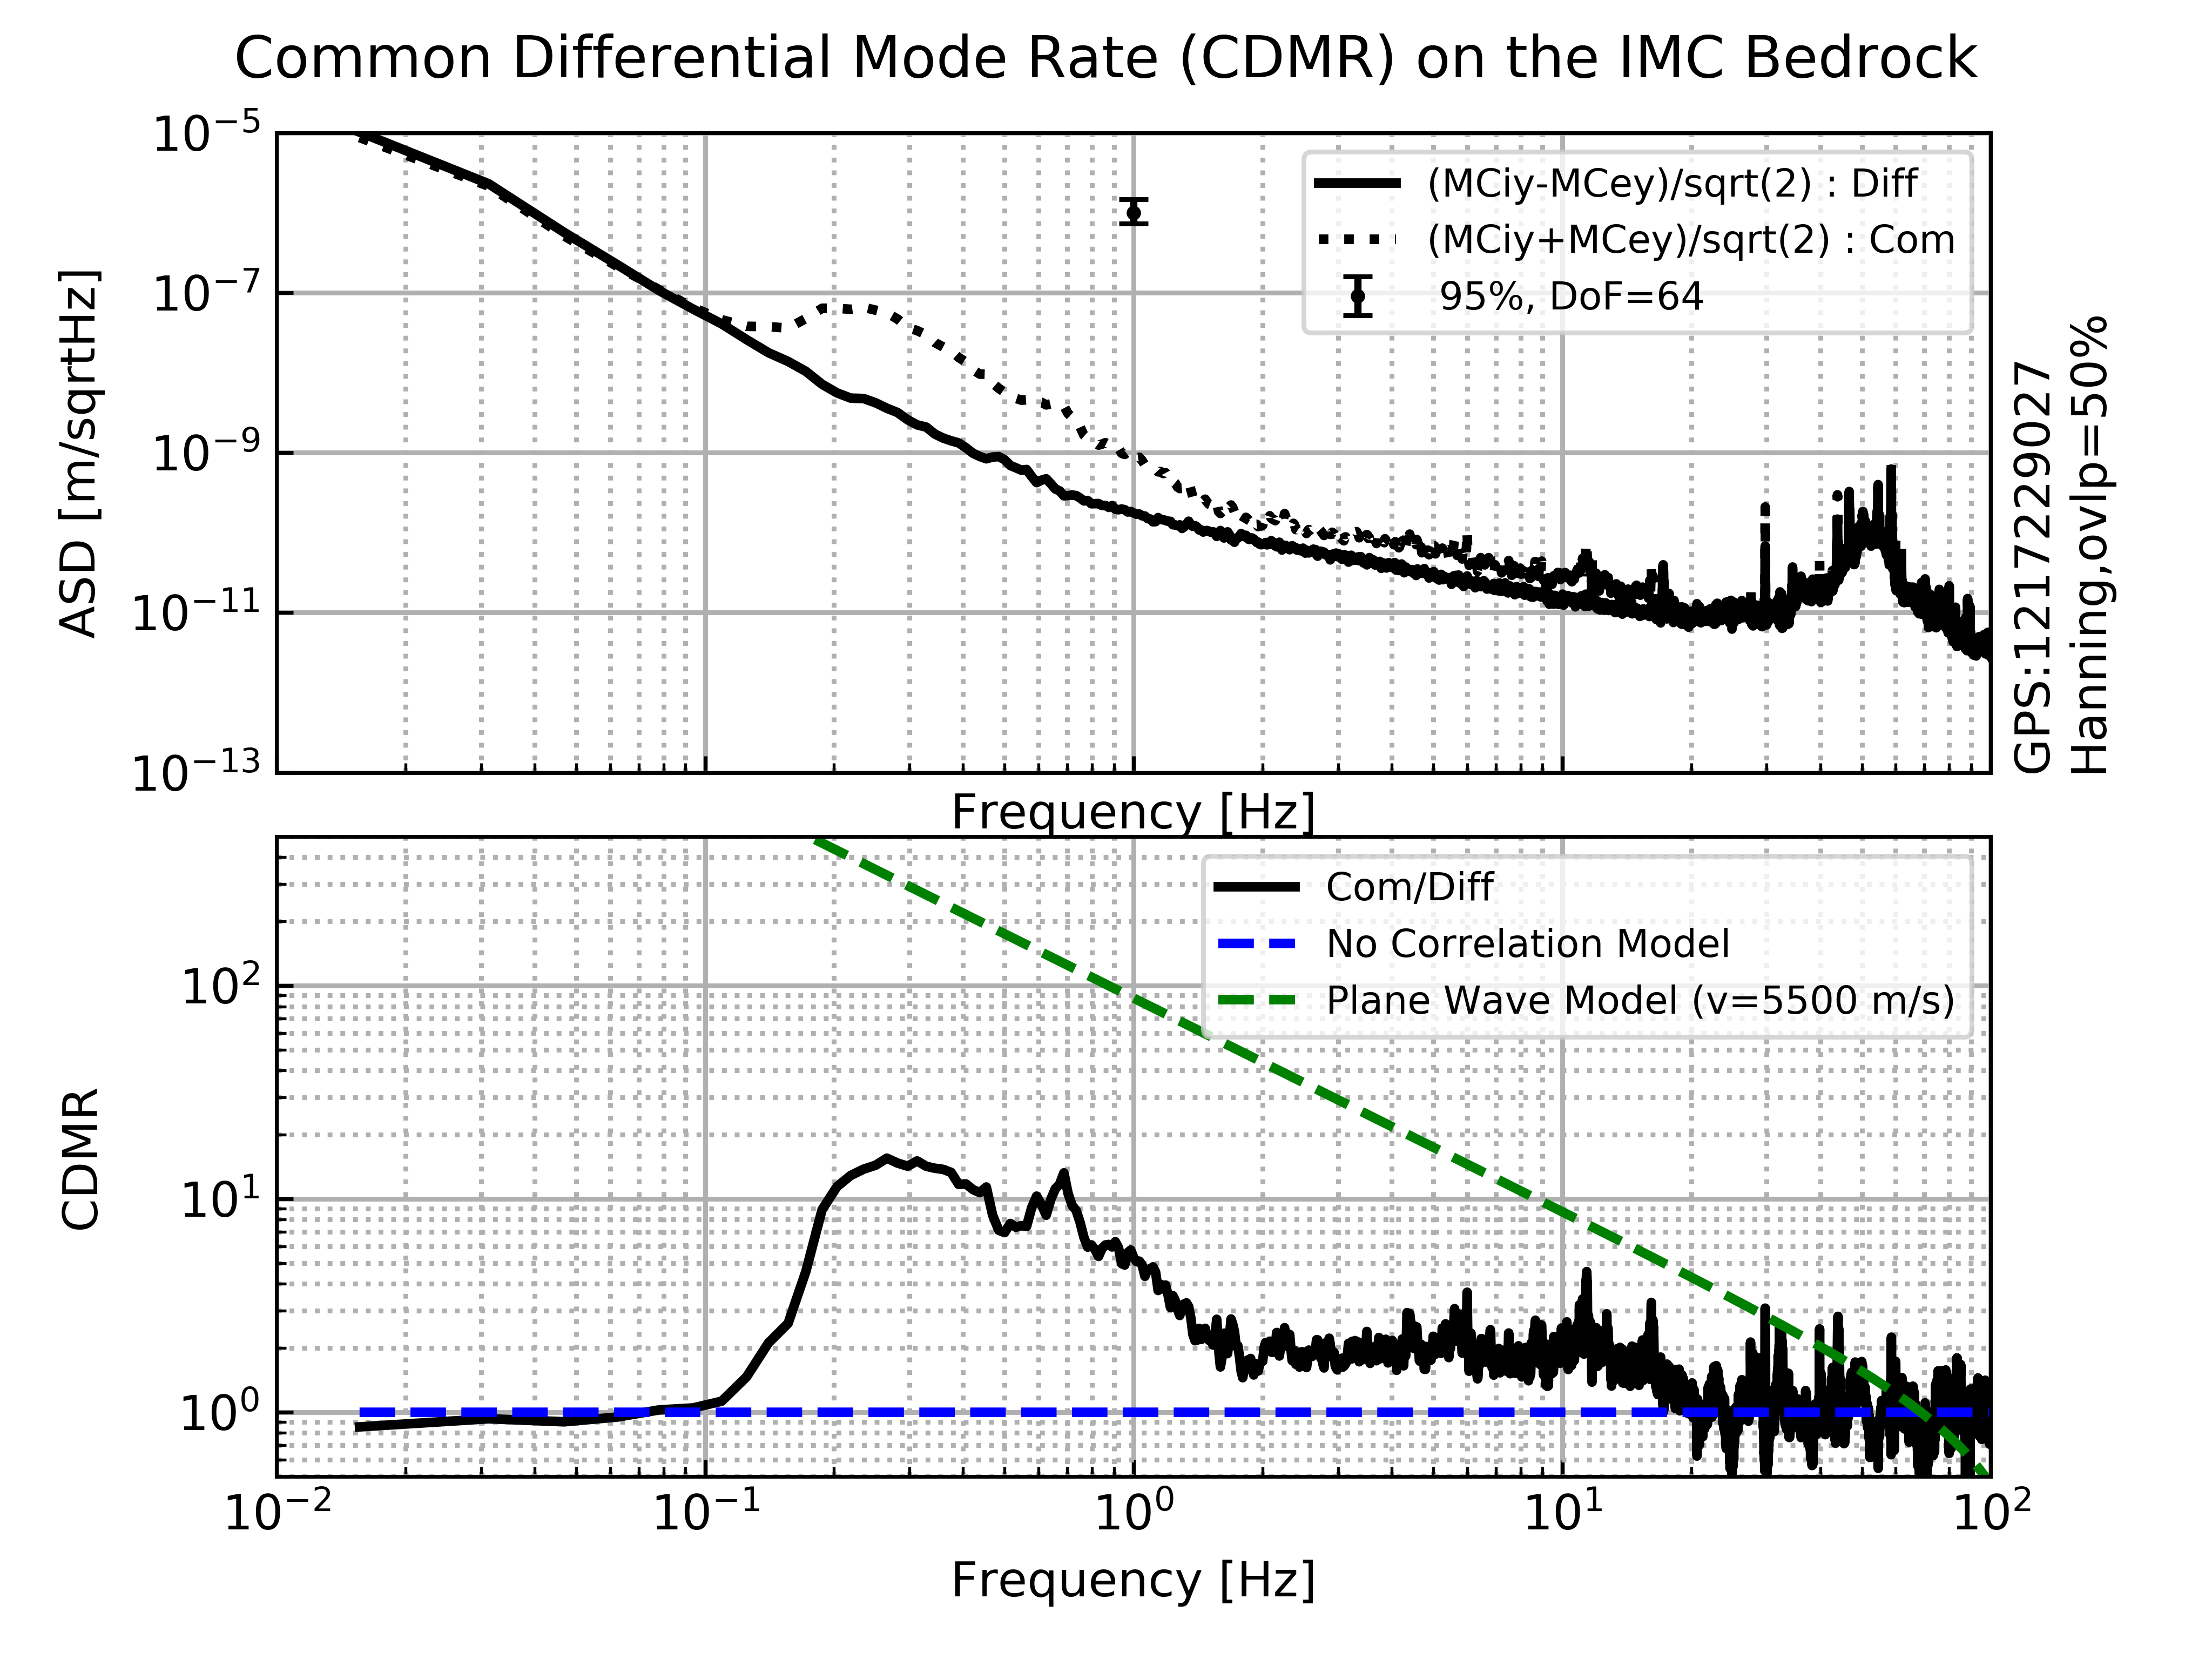
\includegraphics[width=11.5cm]{./img_cdmr_imc.png}
  \end{center}
  \caption{aa}\label{img:img_cdmr_imc}
\end{figure}
図\ref{img:img_cdmr_imc}にCDMRを示す。図\ref{img:img_coherence_imc}で,位相差0度でコヒーレンスのあった帯域では,逆相成分は同相成分よりも小さいことがわかる。図\ref{img:img_cdmr_imc}下の緑色の破線で示している平面波のモデルとは一致していないが,これは,逆相成分が地震計のSelfノイズで埋もれてしまっているからだと考えられる。\footnote[12]{Selfノイズのプロットは後日。個々のSelfノイズは一緒だとして,そのASDを$\sqrt{2}$倍すればいい。(時系列データが神岡のサーバから柏に移動して見れないので,もう一度グラフをつくるのが面倒。)あと,もしくはもともとの無相関な地面振動のノイズレベルで埋もれているのかも。}






\subsection{まとめ}
本章では、同相成分と逆相成分の比であるCommon Differential Mode Ratio (CDMR)という量を定義して,Xアームで脈動はどれだけ逆相成分を低減されているのか,評価した。その結果,最大でCDMRは4あり,逆相成分が同相成分よりも小さくなっていることが確認できた。これは,基線方向を平面波が伝搬するモデルで予想される値とよく一致している。

さらに,この評価をおよそ30mのIMCの基線長についても行った。その結果,CDMRは最大で10あった。この値は平面波のモデルと比較すると,1桁ほど小さい値になっているが,これは地震計のSelfノイズか地面振動のノイズレベルでSNが悪くなっているためだと考えられる。

今後は,いくつかの時期でCDMRをもとめ,基線長伸縮スペクトルの代表値をもとめる。 \footnote[13]{いまの解析コードだと,直近1周間のデータしか解析できない。なので,たとえばこの時期周辺の時系列データを解析しようと思ったら,柏のデータサーバにアクセスしないといけなくなるけど,対応しているデータの読み出しの方法が神岡と柏で違うので解析コードを改良しないといけない。これが結構面倒。}


\appendix
\section{スペクトルの誤差}
\section{コヒーレンスの有意水準}


\bibliography{./cdmr_reference}
